\iftestbuild % TEST-ONLY-BEGIN
\setcounter{section}{2}\setcounter{theorem}{45}
\fi % TEST-ONLY-END
% Source: book pp. 211--226 (PDF 225--240); no solutions.
% Numbered equations (6.50, 6.53, ...): \axeqstep{ax:N.M} steps Axler's counter
% and sets the label just before the display; \axeqtag prints the number.
\DeclareRobustCommand\axeqstep[1]{\refstepcounter{theorem}\label{#1}}
\DeclareRobustCommand\axeqtag{\tag*{\thetheorem}}
\section{Orthogonal Complements and Minimization Problems}

\subsection{Orthogonal Complements}

\begin{definition}[Orthogonal complement, $U^\perp$]\label{ax:6.46}
If $U$ is a subset of $V$, then the \emph{orthogonal complement} of $U$, denoted
by $U^\perp$, is the set of all vectors in $V$ that are orthogonal to every
vector in $U$:
\[ U^\perp = \{v\in V : \ip{u}{v}=0 \text{ for every } u\in U\}. \]
\end{definition}

The orthogonal complement $U^\perp$ depends on $V$ as well as on $U$. However,
the inner product space $V$ should always be clear from the context and thus it
can be omitted from the notation.

\begin{example}[Orthogonal complements]\label{ax:6.47}\leavevmode
\begin{itemize}
\item If $V=\R^3$ and $U$ is the subset of $V$ consisting of the single point
  $(2,3,5)$, then $U^\perp$ is the plane
  $\{(x,y,z)\in\R^3 : 2x+3y+5z=0\}$.
\item If $V=\R^3$ and $U$ is the plane $\{(x,y,z)\in\R^3 : 2x+3y+5z=0\}$, then
  $U^\perp$ is the line $\{(2t,3t,5t) : t\in\R\}$.
\item More generally, if $U$ is a plane in $\R^3$ containing the origin, then
  $U^\perp$ is the line containing the origin that is perpendicular to $U$.
\item If $U$ is a line in $\R^3$ containing the origin, then $U^\perp$ is the
  plane containing the origin that is perpendicular to $U$.
\item If $V=\F^5$ and $U=\{(a,b,0,0,0)\in\F^5 : a,b\in\F\}$, then
  \[ U^\perp = \{(0,0,x,y,z)\in\F^5 : x,y,z\in\F\}. \]
\item If $e_1,\dots,e_m,f_1,\dots,f_n$ is an orthonormal basis of $V$, then
  \[ \bigl(\spn(e_1,\dots,e_m)\bigr)^\perp = \spn(f_1,\dots,f_n). \]
\end{itemize}
\end{example}

We begin with some straightforward consequences of the definition.

\begin{result}[Properties of orthogonal complement]\label{ax:6.48}\leavevmode
\begin{parts}
\item If $U$ is a subset of $V$, then $U^\perp$ is a subspace of $V$.
\item $\{0\}^\perp=V$.
\item $V^\perp=\{0\}$.
\item If $U$ is a subset of $V$, then $U\cap U^\perp\subseteq\{0\}$.
\item If $G$ and $H$ are subsets of $V$ and $G\subseteq H$, then
  $H^\perp\subseteq G^\perp$.
\end{parts}
\end{result}

\begin{proof}\leavevmode
\begin{parts}
\item Suppose $U$ is a subset of $V$. Then $\ip{u}{0}=0$ for every $u\in U$;
  thus $0\in U^\perp$.

  Suppose $v,w\in U^\perp$. If $u\in U$, then
  \[ \ip{u}{v+w} = \ip{u}{v}+\ip{u}{w} = 0+0 = 0. \]
  Thus $v+w\in U^\perp$, which shows that $U^\perp$ is closed under addition.

  Similarly, suppose $\lambda\in\F$ and $v\in U^\perp$. If $u\in U$, then
  \[ \ip{u}{\lambda v} = \overline{\lambda}\ip{u}{v}
     = \overline{\lambda}\cdot0 = 0. \]
  Thus $\lambda v\in U^\perp$, which shows that $U^\perp$ is closed under
  scalar multiplication. Thus $U^\perp$ is a subspace of $V$.
\item Suppose that $v\in V$. Then $\ip{0}{v}=0$, which implies that
  $v\in\{0\}^\perp$. Thus $\{0\}^\perp=V$.
\item Suppose that $v\in V^\perp$. Then $\ip{v}{v}=0$, which implies that
  $v=0$. Thus $V^\perp=\{0\}$.
\item Suppose $U$ is a subset of $V$ and $u\in U\cap U^\perp$. Then
  $\ip{u}{u}=0$, which implies that $u=0$. Thus $U\cap U^\perp\subseteq\{0\}$.
\item Suppose $G$ and $H$ are subsets of $V$ and $G\subseteq H$. Suppose
  $v\in H^\perp$. Then $\ip{u}{v}=0$ for every $u\in H$, which implies that
  $\ip{u}{v}=0$ for every $u\in G$. Hence $v\in G^\perp$. Thus
  $H^\perp\subseteq G^\perp$. \qedhere
\end{parts}
\end{proof}

Recall that if $U$ and $W$ are subspaces of $V$, then $V$ is the direct sum of
$U$ and $W$ (written $V=U\oplus W$) if each element of $V$ can be written in
exactly one way as a vector in $U$ plus a vector in $W$ (see \ref{ax:1.41}).
Furthermore, this happens if and only if $V=U+W$ and $U\cap W=\{0\}$ (see
\ref{ax:1.46}).

The next result shows that every finite-dimensional subspace of $V$ leads to a
natural direct sum decomposition of $V$. See Exercise~16 for an example showing
that the result below can fail without the hypothesis that the subspace $U$ is
finite-dimensional.

\begin{result}[Direct sum of a subspace and its orthogonal
complement]\label{ax:6.49}
Suppose $U$ is a finite-dimensional subspace of $V$. Then
\[ V = U\oplus U^\perp. \]
\end{result}

\begin{proof}
First we will show that
\[ V = U+U^\perp. \]
To do this, suppose that $v\in V$. Let $e_1,\dots,e_m$ be an orthonormal basis
of $U$. We want to write $v$ as the sum of a vector in $U$ and a vector
orthogonal to $U$.

We have\axeqstep{ax:6.50}
\begin{equation*}
v = \underbrace{\ip{v}{e_1}e_1+\cdots+\ip{v}{e_m}e_m}_{u}
  + \underbrace{v-\ip{v}{e_1}e_1-\cdots-\ip{v}{e_m}e_m}_{w}. \axeqtag
\end{equation*}
Let $u$ and $w$ be defined as in the equation above (as was done in the proof
of \ref{ax:6.26}). Because each $e_k\in U$, we see that $u\in U$. Because
$e_1,\dots,e_m$ is an orthonormal list, for each $k=1,\dots,m$ we have
\begin{align*}
\ip{w}{e_k} &= \ip{v}{e_k}-\ip{v}{e_k}\\
            &= 0.
\end{align*}
Thus $w$ is orthogonal to every vector in $\spn(e_1,\dots,e_m)$, which shows
that $w\in U^\perp$. Hence we have written $v=u+w$, where $u\in U$ and
$w\in U^\perp$, completing the proof that $V=U+U^\perp$.

From \ref{ax:6.48}(d), we know that $U\cap U^\perp=\{0\}$. Now equation
$V=U+U^\perp$ implies that $V=U\oplus U^\perp$ (see \ref{ax:1.46}).
\end{proof}

Now we can see how to compute $\dim U^\perp$ from $\dim U$.

\begin{result}[Dimension of orthogonal complement]\label{ax:6.51}
Suppose $V$ is finite-dimensional and $U$ is a subspace of $V$. Then
\[ \dim U^\perp = \dim V - \dim U. \]
\end{result}

\begin{proof}
The formula for $\dim U^\perp$ follows immediately from \ref{ax:6.49} and
\ref{ax:3.94}.
\end{proof}

The next result is an important consequence of \ref{ax:6.49}.

\begin{result}[Orthogonal complement of the orthogonal
complement]\label{ax:6.52}
Suppose $U$ is a finite-dimensional subspace of $V$. Then
\[ U = (U^\perp)^\perp. \]
\end{result}

\begin{proof}
First we will show that\axeqstep{ax:6.53}
\begin{equation*}
U \subseteq (U^\perp)^\perp. \axeqtag
\end{equation*}
To do this, suppose $u\in U$. Then $\ip{u}{w}=0$ for every $w\in U^\perp$ (by
the definition of $U^\perp$). Because $u$ is orthogonal to every vector in
$U^\perp$, we have $u\in(U^\perp)^\perp$, completing the proof of
\ref{ax:6.53}.

To prove the inclusion in the other direction, suppose
$v\in(U^\perp)^\perp$. By \ref{ax:6.49}, we can write $v=u+w$, where $u\in U$
and $w\in U^\perp$. We have $v-u=w\in U^\perp$. Because $v\in(U^\perp)^\perp$
and $u\in(U^\perp)^\perp$ (from \ref{ax:6.53}), we have
$v-u\in(U^\perp)^\perp$. Thus $v-u\in U^\perp\cap(U^\perp)^\perp$, which
implies that $v-u=0$ [by \ref{ax:6.48}(d)], which implies that $v=u$, which
implies that $v\in U$. Thus $(U^\perp)^\perp\subseteq U$, which along with
\ref{ax:6.53} completes the proof.
\end{proof}

\marginnote{Exercise~16(a) shows that the result below is not true without the
hypothesis that $U$ is finite-dimensional.}%
Suppose $U$ is a subspace of $V$ and we want to show that $U=V$. In some
situations, the easiest way to do this is to show that the only vector
orthogonal to $U$ is $0$, and then use the result below. For example, the
result below is useful for Exercise~4.

\begin{result}[$U^\perp=\{0\}\iff U=V$ (for $U$ a finite-dimensional subspace
of $V$)]\label{ax:6.54}
Suppose $U$ is a finite-dimensional subspace of $V$. Then
\[ U^\perp=\{0\} \iff U=V. \]
\end{result}

\begin{proof}
First suppose $U^\perp=\{0\}$. Then by \ref{ax:6.52},
$U=(U^\perp)^\perp=\{0\}^\perp=V$, as desired.

Conversely, if $U=V$, then $U^\perp=V^\perp=\{0\}$ by \ref{ax:6.48}(c).
\end{proof}

We now define an operator $P_U$ for each finite-dimensional subspace $U$ of
$V$.

\begin{definition}[Orthogonal projection, $P_U$]\label{ax:6.55}
Suppose $U$ is a finite-dimensional subspace of $V$. The \emph{orthogonal
projection} of $V$ onto $U$ is the operator $P_U\in\Lin(V)$ defined as follows:
For each $v\in V$, write $v=u+w$, where $u\in U$ and $w\in U^\perp$. Then let
$P_Uv=u$.
\end{definition}

The direct sum decomposition $V=U\oplus U^\perp$ given by \ref{ax:6.49} shows
that each $v\in V$ can be uniquely written in the form $v=u+w$ with $u\in U$
and $w\in U^\perp$. Thus $P_Uv$ is well defined. See the figure that
accompanies the proof of \ref{ax:6.61} for the picture describing $P_Uv$ that
you should keep in mind.

\begin{example}[Orthogonal projection onto one-dimensional
subspace]\label{ax:6.56}
Suppose $u\in V$ with $u\ne0$ and $U$ is the one-dimensional subspace of $V$
defined by $U=\spn(u)$.

If $v\in V$, then
\[ v = \frac{\ip{v}{u}}{\norm{u}^2}u
     + \biggl(v-\frac{\ip{v}{u}}{\norm{u}^2}u\biggr), \]
where the first term on the right is in $\spn(u)$ (and thus is in $U$) and the
second term on the right is orthogonal to $u$ (and thus is in $U^\perp$). Thus
$P_Uv$ equals the first term on the right. In other words, we have the formula
\[ P_Uv = \frac{\ip{v}{u}}{\norm{u}^2}u \]
for every $v\in V$.

The formula above becomes $P_Uu=u$ if $v=u$ and becomes $P_Uv=0$ if
$v\in\{u\}^\perp$. These equations are special cases of (b) and (c) in the next
result.
\end{example}

\begin{result}[Properties of orthogonal projection $P_U$]\label{ax:6.57}
Suppose $U$ is a finite-dimensional subspace of $V$. Then
\begin{parts}
\item $P_U\in\Lin(V)$;
\item $P_Uu=u$ for every $u\in U$;
\item $P_Uw=0$ for every $w\in U^\perp$;
\item $\range P_U=U$;
\item $\nul P_U=U^\perp$;
\item $v-P_Uv\in U^\perp$ for every $v\in V$;
\item $P_U^2=P_U$;
\item $\norm{P_Uv}\le\norm{v}$ for every $v\in V$;
\item if $e_1,\dots,e_m$ is an orthonormal basis of $U$ and $v\in V$, then
  \[ P_Uv = \ip{v}{e_1}e_1+\cdots+\ip{v}{e_m}e_m. \]
\end{parts}
\end{result}

\begin{proof}\leavevmode
\begin{parts}
\item To show that $P_U$ is a linear map on $V$, suppose $v_1,v_2\in V$. Write
  \[ v_1=u_1+w_1 \quad\text{and}\quad v_2=u_2+w_2 \]
  with $u_1,u_2\in U$ and $w_1,w_2\in U^\perp$. Thus $P_Uv_1=u_1$ and
  $P_Uv_2=u_2$. Now
  \[ v_1+v_2 = (u_1+u_2)+(w_1+w_2), \]
  where $u_1+u_2\in U$ and $w_1+w_2\in U^\perp$. Thus
  \[ P_U(v_1+v_2) = u_1+u_2 = P_Uv_1+P_Uv_2. \]

  Similarly, suppose $\lambda\in\F$ and $v\in V$. Write $v=u+w$, where $u\in U$
  and $w\in U^\perp$. Then $\lambda v=\lambda u+\lambda w$ with
  $\lambda u\in U$ and $\lambda w\in U^\perp$. Thus
  $P_U(\lambda v)=\lambda u=\lambda P_Uv$.

  Hence $P_U$ is a linear map from $V$ to $V$.
\item Suppose $u\in U$. We can write $u=u+0$, where $u\in U$ and
  $0\in U^\perp$. Thus $P_Uu=u$.
\item Suppose $w\in U^\perp$. We can write $w=0+w$, where $0\in U$ and
  $w\in U^\perp$. Thus $P_Uw=0$.
\item The definition of $P_U$ implies that $\range P_U\subseteq U$.
  Furthermore, (b) implies that $U\subseteq\range P_U$. Thus $\range P_U=U$.
\item The inclusion $U^\perp\subseteq\nul P_U$ follows from (c). To prove the
  inclusion in the other direction, note that if $v\in\nul P_U$ then the
  decomposition given by \ref{ax:6.49} must be $v=0+v$, where $0\in U$ and
  $v\in U^\perp$. Thus $\nul P_U\subseteq U^\perp$.
\item If $v\in V$ and $v=u+w$ with $u\in U$ and $w\in U^\perp$, then
  \[ v-P_Uv = v-u = w\in U^\perp. \]
\item If $v\in V$ and $v=u+w$ with $u\in U$ and $w\in U^\perp$, then
  \[ (P_U^2)v = P_U(P_Uv) = P_Uu = u = P_Uv. \]
\item If $v\in V$ and $v=u+w$ with $u\in U$ and $w\in U^\perp$, then
  \[ \norm{P_Uv}^2 = \norm{u}^2 \le \norm{u}^2+\norm{w}^2 = \norm{v}^2, \]
  where the last equality comes from the Pythagorean theorem.
\item The formula for $P_Uv$ follows from equation \ref{ax:6.50} in the proof
  of \ref{ax:6.49}. \qedhere
\end{parts}
\end{proof}

In the previous section we proved the Riesz representation theorem
(\ref{ax:6.42}), whose key part states that every linear functional on a
finite-dimensional inner product space is given by taking the inner product
with some fixed vector. Seeing a different proof often provides new insight.
Thus we now give a new proof of the key part of the Riesz representation
theorem using orthogonal complements instead of orthonormal bases as in our
previous proof.

The restatement below of the Riesz representation theorem provides an
identification of $V$ with $V'$. We will prove only the ``onto'' part of the
result below because the more routine ``one-to-one'' part of the result can be
proved as in \ref{ax:6.42}.

Intuition behind this new proof: If $\varphi\in V'$, $v\in V$, and
$\varphi(u)=\ip{u}{v}$ for all $u\in V$, then $v\in(\nul\varphi)^\perp$.
However, $(\nul\varphi)^\perp$ is a one-dimensional subspace of $V$ (except for
the trivial case in which $\varphi=0$), as follows from \ref{ax:6.51} and
\ref{ax:3.21}. Thus we can obtain $v$ by choosing any nonzero element of
$(\nul\varphi)^\perp$ and then multiplying by an appropriate scalar, as is done
in the proof below.

\begin{result}[Riesz representation theorem, revisited]\label{ax:6.58}
Suppose $V$ is finite-dimensional. For each $v\in V$, define
$\varphi_v\in V'$ by
\[ \varphi_v(u) = \ip{u}{v} \]
for each $u\in V$. Then $v\mapsto\varphi_v$ is a one-to-one function from $V$
onto $V'$.
\end{result}

\marginnote[11mm]{\textbf{Caution:} The function $v\mapsto\varphi_v$ is a linear
mapping from $V$ to $V'$ if $\F=\R$. However, this function is not linear if
$\F=\C$ because $\varphi_{\lambda v}=\overline{\lambda}\varphi_v$ if
$\lambda\in\C$.}%
\begin{proof}
To show that $v\mapsto\varphi_v$ is surjective, suppose $\varphi\in V'$. If
$\varphi=0$, then $\varphi=\varphi_0$. Thus assume $\varphi\ne0$. Hence
$\nul\varphi\ne V$, which implies that $(\nul\varphi)^\perp\ne\{0\}$ (by
\ref{ax:6.49} with $U=\nul\varphi$).

Let $w\in(\nul\varphi)^\perp$ be such that $w\ne0$. Let\axeqstep{ax:6.59}
\begin{equation*}
v = \frac{\overline{\varphi(w)}}{\norm{w}^2}w. \axeqtag
\end{equation*}
Then $v\in(\nul\varphi)^\perp$. Also, $v\ne0$ (because
$w\notin\nul\varphi$).

Taking the norm of both sides of \ref{ax:6.59} gives\axeqstep{ax:6.60}
\begin{equation*}
\norm{v} = \frac{\abs{\varphi(w)}}{\norm{w}}. \axeqtag
\end{equation*}
Applying $\varphi$ to both sides of \ref{ax:6.59} and then using
\ref{ax:6.60}, we have
\[ \varphi(v) = \frac{\abs{\varphi(w)}^2}{\norm{w}^2} = \norm{v}^2. \]

Now suppose $u\in V$. Using the equation above, we have
\[ u = \biggl(u-\frac{\varphi(u)}{\varphi(v)}v\biggr)
     + \frac{\varphi(u)}{\norm{v}^2}v. \]
The first term in parentheses above is in $\nul\varphi$ and hence is orthogonal
to $v$. Thus taking the inner product of both sides of the equation above with
$v$ shows that
\[ \ip{u}{v} = \frac{\varphi(u)}{\norm{v}^2}\ip{v}{v} = \varphi(u). \]
Thus $\varphi=\varphi_v$, showing that $v\mapsto\varphi_v$ is surjective, as
desired.
\end{proof}

See Exercise~13 for yet another proof of the Riesz representation theorem.

\subsection{Minimization Problems}

\marginnote{The remarkable simplicity of the solution to this minimization
problem has led to many important applications of inner product spaces outside
of pure mathematics.}%
The following problem often arises: Given a subspace $U$ of $V$ and a point
$v\in V$, find a point $u\in U$ such that $\norm{v-u}$ is as small as possible.
The next result shows that $u=P_Uv$ is the unique solution of this minimization
problem.

\begin{result}[Minimizing distance to a subspace]\label{ax:6.61}
Suppose $U$ is a finite-dimensional subspace of $V$, $v\in V$, and $u\in U$.
Then
\[ \norm{v-P_Uv} \le \norm{v-u}. \]
Furthermore, the inequality above is an equality if and only if $u=P_Uv$.
\end{result}

\begin{proof}
We have\axeqstep{ax:6.62}
\begin{align*}
\norm{v-P_Uv}^2 &\le \norm{v-P_Uv}^2+\norm{P_Uv-u}^2 \axeqtag\\
  &= \bigl\lVert(v-P_Uv)+(P_Uv-u)\bigr\rVert^2\\
  &= \norm{v-u}^2,
\end{align*}
\marginfig{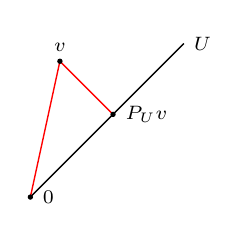
\begin{tikzpicture}[scale=.75]
  \draw[line width=.5pt] (0,0)--(2.6,2.6) node[right,font=\scriptsize] {$U$};
  \draw[red,line width=.5pt] (0,0)--(.5,2.3)--(1.4,1.4);
  \fill (0,0) circle (1.3pt) node[right=1pt,font=\scriptsize] {$0$};
  \fill (.5,2.3) circle (1.3pt) node[above,font=\scriptsize] {$v$};
  \fill (1.4,1.4) circle (1.3pt) node[right=1pt,font=\scriptsize] {$P_Uv$};
\end{tikzpicture}}{$P_Uv$ is the closest point in $U$ to $v$.}%
where the first line above holds because $0\le\norm{P_Uv-u}^2$, the second line
above comes from the Pythagorean theorem [which applies because
$v-P_Uv\in U^\perp$ by \ref{ax:6.57}(f), and $P_Uv-u\in U$], and the third line
above holds by simple algebra. Taking square roots gives the desired
inequality.

The inequality proved above is an equality if and only if \ref{ax:6.62} is an
equality, which happens if and only if $\norm{P_Uv-u}=0$, which happens if and
only if $u=P_Uv$.
\end{proof}

The last result is often combined with the formula \ref{ax:6.57}(i) to compute
explicit solutions to minimization problems, as in the following example.

\begin{example}[Using linear algebra to approximate the sine
function]\label{ax:6.63}
Suppose we want to find a polynomial $u$ with real coefficients and of degree
at most $5$ that approximates the sine function as well as possible on the
interval $[-\pi,\pi]$, in the sense that
\[ \int_{-\pi}^{\pi} \abs{\sin x-u(x)}^2\,dx \]
is as small as possible.

Let $C[-\pi,\pi]$ denote the real inner product space of continuous real-valued
functions on $[-\pi,\pi]$ with inner product\axeqstep{ax:6.64}
\begin{equation*}
\ip{f}{g} = \int_{-\pi}^{\pi} fg. \axeqtag
\end{equation*}
Let $v\in C[-\pi,\pi]$ be the function defined by $v(x)=\sin x$. Let $U$ denote
the subspace of $C[-\pi,\pi]$ consisting of the polynomials with real
coefficients and of degree at most $5$. Our problem can now be reformulated as
follows:
\[ \text{Find } u\in U \text{ such that } \norm{v-u}
   \text{ is as small as possible.} \]

To compute the solution to our approximation problem, first apply the
Gram--Schmidt procedure (using the inner product given by \ref{ax:6.64}) to the
basis $1,x,x^2,x^3,x^4,x^5$ of $U$, producing an orthonormal basis
$e_1,e_2,e_3,e_4,e_5,e_6$ of $U$. Then, again using the inner product given by
\ref{ax:6.64}, compute $P_Uv$ using \ref{ax:6.57}(i) (with $m=6$). Doing this
computation shows that $P_Uv$ is the function $u$ defined
by\axeqstep{ax:6.65}
\begin{equation*}
u(x) = 0.987862x-0.155271x^3+0.00564312x^5, \axeqtag
\end{equation*}
where the $\pi$'s that appear in the exact answer have been replaced with a
good decimal approximation. By \ref{ax:6.61}, the polynomial $u$ above is the
best approximation to the sine function on $[-\pi,\pi]$ using polynomials of
degree at most $5$ (here ``best approximation'' means in the sense of
minimizing $\int_{-\pi}^{\pi}\abs{\sin x-u(x)}^2\,dx$).

To see how good this approximation is, the next figure shows the graphs of both
the sine function and our approximation $u$ given by \ref{ax:6.65} over the
interval $[-\pi,\pi]$.
\begin{center}
\begin{tikzpicture}[xscale=1.2,yscale=1]
  \draw[line width=.4pt] (-3.3,0)--(3.3,0);
  \draw[line width=.4pt] (0,-1.15)--(0,1.15);
  \foreach \y in {-1,1} \draw (0,\y)--(-.06,\y) node[left,font=\scriptsize]
    {$\y$};
  \foreach \x/\l in {-pi/-\pi,pi/\pi} \draw (\x,0)--(\x,-.06)
    node[below,font=\scriptsize] {$\l$};
  \draw[blue,line width=.6pt,domain=-pi:pi,samples=120]
    plot (\x,{0.987862*\x-0.155271*\x^3+0.00564312*\x^5});
  \draw[red,line width=.6pt,domain=-pi:pi,samples=120] plot (\x,{sin(\x r)});
\end{tikzpicture}
\captionof*{figure}{Graphs on $[-\pi,\pi]$ of the sine function (red) and its
best fifth degree polynomial approximation $u$ (blue) from \ref{ax:6.65}.}
\end{center}

Our approximation \ref{ax:6.65} is so accurate that the two graphs are almost
identical---our eyes may see only one graph! Here the red graph is placed
almost exactly over the blue graph. If you are viewing this on an electronic
device, enlarge the picture above by 400\% near $\pi$ or $-\pi$ to see a small
gap between the two graphs.

Another well-known approximation to the sine function by a polynomial of degree
$5$ is given by the Taylor polynomial $p$ defined by\axeqstep{ax:6.66}
\begin{equation*}
p(x) = x-\frac{x^3}{3!}+\frac{x^5}{5!}. \axeqtag
\end{equation*}
To see how good this approximation is, the next picture shows the graphs of
both the sine function and the Taylor polynomial $p$ over the interval
$[-\pi,\pi]$.
\begin{center}
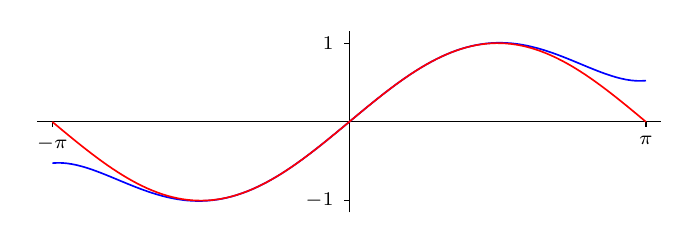
\begin{tikzpicture}[xscale=1.2,yscale=1]
  \draw[line width=.4pt] (-3.3,0)--(3.3,0);
  \draw[line width=.4pt] (0,-1.15)--(0,1.15);
  \foreach \y in {-1,1} \draw (0,\y)--(-.06,\y) node[left,font=\scriptsize]
    {$\y$};
  \foreach \x/\l in {-pi/-\pi,pi/\pi} \draw (\x,0)--(\x,-.06)
    node[below,font=\scriptsize] {$\l$};
  \draw[blue,line width=.6pt,domain=-pi:pi,samples=120]
    plot (\x,{\x-\x^3/6+\x^5/120});
  \draw[red,line width=.6pt,domain=-pi:pi,samples=120] plot (\x,{sin(\x r)});
\end{tikzpicture}
\captionof*{figure}{Graphs on $[-\pi,\pi]$ of the sine function (red) and the
Taylor polynomial (blue) from \ref{ax:6.66}.}
\end{center}

The Taylor polynomial of degree $5$ is an excellent approximation to $\sin x$
for $x$ near $0$. But the picture above shows that for $\abs{x}>2$, the Taylor
polynomial is not so accurate, especially compared to \ref{ax:6.65}. For
example, taking $x=3$, our approximation \ref{ax:6.65} estimates $\sin 3$ with
an error of approximately $0.001$, but the Taylor polynomial \ref{ax:6.66}
estimates $\sin 3$ with an error of approximately $0.4$. Thus at $x=3$, the
error in the Taylor polynomial is hundreds of times larger than the error given
by \ref{ax:6.65}. Linear algebra has helped us discover an approximation to the
sine function that improves upon what we learned in calculus!
\end{example}

\subsection{Pseudoinverse}

Suppose $T\in\Lin(V,W)$ and $w\in W$. Consider the problem of finding $v\in V$
such that
\[ Tv = w. \]
For example, if $V=\F^n$ and $W=\F^m$, then the equation above could represent
a system of $m$ linear equations in $n$ unknowns $v_1,\dots,v_n$, where
$v=(v_1,\dots,v_n)$.

If $T$ is invertible, then the unique solution to the equation above is
$v=T^{-1}w$. However, if $T$ is not invertible, then for some $w\in W$ there
may not exist any solutions of the equation above, and for some $w\in W$ there
may exist infinitely many solutions of the equation above.

If $T$ is not invertible, then we can still try to do as well as possible with
the equation above. For example, if the equation above has no solutions, then
instead of solving the equation $Tv-w=0$, we can try to find $v\in V$ such that
$\norm{Tv-w}$ is as small as possible. As another example, if the equation
above has infinitely many solutions $v\in V$, then among all those solutions we
can try to find one such that $\norm{v}$ is as small as possible.

The pseudoinverse will provide the tool to solve the equation above as well as
possible, even when $T$ is not invertible. We need the next result to define
the pseudoinverse.

In the next two proofs, we will use without further comment the result that if
$V$ is finite-dimensional and $T\in\Lin(V,W)$, then $\nul T$,
$(\nul T)^\perp$, and $\range T$ are all finite-dimensional.

\begin{result}[Restriction of a linear map to obtain a one-to-one and onto
map]\label{ax:6.67}
Suppose $V$ is finite-dimensional and $T\in\Lin(V,W)$. Then
$T|_{(\nul T)^\perp}$ is an injective map of $(\nul T)^\perp$ onto $\range T$.
\end{result}

\begin{proof}
Suppose that $v\in(\nul T)^\perp$ and $T|_{(\nul T)^\perp}v=0$. Hence $Tv=0$
and thus $v\in(\nul T)\cap(\nul T)^\perp$, which implies that $v=0$ [by
\ref{ax:6.48}(d)]. Hence $\nul\bigl(T|_{(\nul T)^\perp}\bigr)=\{0\}$, which
implies that $T|_{(\nul T)^\perp}$ is injective, as desired.

Clearly $\range\bigl(T|_{(\nul T)^\perp}\bigr)\subseteq\range T$. To prove the
inclusion in the other direction, suppose $w\in\range T$. Hence there exists
$v\in V$ such that $w=Tv$. There exist $u\in\nul T$ and $x\in(\nul T)^\perp$
such that $v=u+x$ (by \ref{ax:6.49}). Now
\[ T|_{(\nul T)^\perp}x = Tx = Tv-Tu = w-0 = w, \]
which shows that $w\in\range T|_{(\nul T)^\perp}$. Hence
$\range T\subseteq\range T|_{(\nul T)^\perp}$, completing the proof that
$\range T|_{(\nul T)^\perp}=\range T$.
\end{proof}

\marginnote{To produce the pseudoinverse notation $T^\dagger$ in \TeX, type
\texttt{T\textasciicircum\textbackslash dagger}.}%
Now we can define the pseudoinverse $T^\dagger$ (pronounced ``$T$ dagger'') of
a linear map $T$. In the next definition (and from now on), think of
$T|_{(\nul T)^\perp}$ as an invertible linear map from $(\nul T)^\perp$ onto
$\range T$, as is justified by the result above.

\begin{definition}[Pseudoinverse, $T^\dagger$]\label{ax:6.68}
Suppose that $V$ is finite-dimensional and $T\in\Lin(V,W)$. The
\emph{pseudoinverse} $T^\dagger\in\Lin(W,V)$ of $T$ is the linear map from $W$
to $V$ defined by
\[ T^\dagger w = \bigl(T|_{(\nul T)^\perp}\bigr)^{-1}P_{\range T}w \]
for each $w\in W$.
\end{definition}

Recall that $P_{\range T}w=0$ if $w\in(\range T)^\perp$ and
$P_{\range T}w=w$ if $w\in\range T$. Thus if $w\in(\range T)^\perp$, then
$T^\dagger w=0$, and if $w\in\range T$, then $T^\dagger w$ is the unique
element of $(\nul T)^\perp$ such that $T(T^\dagger w)=w$.

The pseudoinverse behaves much like an inverse, as we will see.

\begin{result}[Algebraic properties of the pseudoinverse]\label{ax:6.69}
Suppose $V$ is finite-dimensional and $T\in\Lin(V,W)$.
\begin{parts}
\item If $T$ is invertible, then $T^\dagger=T^{-1}$.
\item $TT^\dagger=P_{\range T}=$ the orthogonal projection of $W$ onto
  $\range T$.
\item $T^\dagger T=P_{(\nul T)^\perp}=$ the orthogonal projection of $V$ onto
  $(\nul T)^\perp$.
\end{parts}
\end{result}

\begin{proof}\leavevmode
\begin{parts}
\item Suppose $T$ is invertible. Then $(\nul T)^\perp=V$ and $\range T=W$.
  Thus $T|_{(\nul T)^\perp}=T$ and $P_{\range T}$ is the identity operator on
  $W$. Hence $T^\dagger=T^{-1}$.
\item Suppose $w\in\range T$. Thus
  \[ TT^\dagger w = T\bigl(T|_{(\nul T)^\perp}\bigr)^{-1}w = w
     = P_{\range T}w. \]
  If $w\in(\range T)^\perp$, then $T^\dagger w=0$. Hence
  $TT^\dagger w=0=P_{\range T}w$. Thus $TT^\dagger$ and $P_{\range T}$ agree on
  $\range T$ and on $(\range T)^\perp$. Hence these two linear maps are equal
  (by \ref{ax:6.49}).
\item Suppose $v\in(\nul T)^\perp$. Because $Tv\in\range T$, the definition of
  $T^\dagger$ shows that
  \[ T^\dagger(Tv) = \bigl(T|_{(\nul T)^\perp}\bigr)^{-1}(Tv) = v
     = P_{(\nul T)^\perp}v. \]
  If $v\in\nul T$, then $T^\dagger Tv=0=P_{(\nul T)^\perp}v$. Thus
  $T^\dagger T$ and $P_{(\nul T)^\perp}$ agree on $(\nul T)^\perp$ and on
  $\nul T$. Hence these two linear maps are equal (by \ref{ax:6.49}).
  \qedhere
\end{parts}
\end{proof}

\marginnote{The pseudoinverse is also called the Moore--Penrose inverse.}%
Suppose that $T\in\Lin(V,W)$. If $T$ is surjective, then $TT^\dagger$ is the
identity operator on $W$, as follows from (b) in the result above. If $T$ is
injective, then $T^\dagger T$ is the identity operator on $V$, as follows from
(c) in the result above. For additional algebraic properties of the
pseudoinverse, see Exercises 19--23.

For $T\in\Lin(V,W)$ and $w\in W$, we now return to the problem of finding
$v\in V$ that solves the equation
\[ Tv = w. \]
As we noted earlier, if $T$ is invertible, then $v=T^{-1}w$ is the unique
solution, but if $T$ is not invertible, then $T^{-1}$ is not defined. However,
the pseudoinverse $T^\dagger$ is defined. Taking $v=T^\dagger w$ makes $Tv$ as
close to $w$ as possible, as shown by (a) of the next result. Thus the
pseudoinverse provides what is called a \emph{best fit} to the equation above.

Among all vectors $v\in V$ that make $Tv$ as close as possible to $w$, the
vector $T^\dagger w$ has the smallest norm, as shown by combining (b) in the
next result with the condition for equality in (a).

\begin{result}[Pseudoinverse provides best approximate solution or best
solution]\label{ax:6.70}
Suppose $V$ is finite-dimensional, $T\in\Lin(V,W)$, and $w\in W$.
\begin{parts}
\item If $v\in V$, then
  \[ \bigl\lVert T(T^\dagger w)-w\bigr\rVert \le \norm{Tv-w}, \]
  with equality if and only if $v\in T^\dagger w+\nul T$.
\item If $v\in T^\dagger w+\nul T$, then
  \[ \bigl\lVert T^\dagger w\bigr\rVert \le \norm{v}, \]
  with equality if and only if $v=T^\dagger w$.
\end{parts}
\end{result}

\begin{proof}\leavevmode
\begin{parts}
\item Suppose $v\in V$. Then
  \[ Tv-w = (Tv-TT^\dagger w)+(TT^\dagger w-w). \]
  The first term in parentheses above is in $\range T$. Because the operator
  $TT^\dagger$ is the orthogonal projection of $W$ onto $\range T$ [by
  \ref{ax:6.69}(b)], the second term in parentheses above is in
  $(\range T)^\perp$ [see \ref{ax:6.57}(f)].

  Thus the Pythagorean theorem implies the desired inequality that the norm of
  the second term in parentheses above is less than or equal to
  $\norm{Tv-w}$, with equality if and only if the first term in parentheses
  above equals $0$. Hence we have equality if and only if
  $v-T^\dagger w\in\nul T$, which is equivalent to the statement that
  $v\in T^\dagger w+\nul T$, completing the proof of (a).
\item Suppose $v\in T^\dagger w+\nul T$. Hence $v-T^\dagger w\in\nul T$. Now
  \[ v = (v-T^\dagger w)+T^\dagger w. \]
  The definition of $T^\dagger$ implies that $T^\dagger w\in(\nul T)^\perp$.
  Thus the Pythagorean theorem implies that
  $\bigl\lVert T^\dagger w\bigr\rVert\le\norm{v}$, with equality if and only
  if $v=T^\dagger w$. \qedhere
\end{parts}
\end{proof}

A formula for $T^\dagger$ will be given in the next chapter (see
\ref{ax:7.78}).

\begin{example}[Pseudoinverse of a linear map from $\F^4$ to
$\F^3$]\label{ax:6.71}
Suppose $T\in\Lin(\F^4,\F^3)$ is defined by
\[ T(a,b,c,d) = (a+b+c,\,2c+d,\,0). \]
This linear map is neither injective nor surjective, but we can compute its
pseudoinverse. To do this, first note that
$\range T=\{(x,y,0) : x,y\in\F\}$. Thus
\[ P_{\range T}(x,y,z) = (x,y,0) \]
for each $(x,y,z)\in\F^3$. Also,
\[ \nul T = \{(a,b,c,d)\in\F^4 : a+b+c=0 \text{ and } 2c+d=0\}. \]
The list $(-1,1,0,0)$, $(-1,0,1,-2)$ of two vectors in $\nul T$ spans $\nul T$
because if $(a,b,c,d)\in\nul T$ then
\[ (a,b,c,d) = b(-1,1,0,0)+c(-1,0,1,-2). \]
Because the list $(-1,1,0,0)$, $(-1,0,1,-2)$ is linearly independent, this list
is a basis of $\nul T$.

Now suppose $(x,y,z)\in\F^3$. Then\axeqstep{ax:6.72}
\begin{equation*}
T^\dagger(x,y,z) = \bigl(T|_{(\nul T)^\perp}\bigr)^{-1}P_{\range T}(x,y,z)
  = \bigl(T|_{(\nul T)^\perp}\bigr)^{-1}(x,y,0). \axeqtag
\end{equation*}
The right side of the equation above is the vector $(a,b,c,d)\in\F^4$ such that
$T(a,b,c,d)=(x,y,0)$ and $(a,b,c,d)\in(\nul T)^\perp$. In other words,
$a,b,c,d$ must satisfy the following equations:
\begin{align*}
a+b+c &= x\\
2c+d &= y\\
-a+b &= 0\\
-a+c-2d &= 0,
\end{align*}
where the first two equations are equivalent to the equation
$T(a,b,c,d)=(x,y,0)$ and the last two equations come from the condition for
$(a,b,c,d)$ to be orthogonal to each of the basis vectors $(-1,1,0,0)$,
$(-1,0,1,-2)$ in this basis of $\nul T$. Thinking of $x$ and $y$ as constants
and $a$, $b$, $c$, $d$ as unknowns, we can solve the system above of four
equations in four unknowns, getting
\[ a=(1/11)(5x-2y),\ b=(1/11)(5x-2y),\
   c=(1/11)(x+4y),\ d=(1/11)(-2x+3y). \]
Hence \ref{ax:6.72} tells us that
\[ T^\dagger(x,y,z) = (1/11)(5x-2y,\,5x-2y,\,x+4y,\,-2x+3y). \]
The formula above for $T^\dagger$ shows that $TT^\dagger(x,y,z)=(x,y,0)$ for
all $(x,y,z)\in\F^3$, which illustrates the equation $TT^\dagger=P_{\range T}$
from \ref{ax:6.69}(b).
\end{example}

% ------------------------------------------------------------------ exercises
\begin{exc}

\begin{exercise}
Suppose $v_1,\dots,v_m\in V$. Prove that
\[ \{v_1,\dots,v_m\}^\perp = \bigl(\spn(v_1,\dots,v_m)\bigr)^\perp. \]
\end{exercise}

\begin{exercise}
Suppose $U$ is a subspace of $V$ with basis $u_1,\dots,u_m$ and
\[ u_1,\dots,u_m,v_1,\dots,v_n \]
is a basis of $V$. Prove that if the Gram--Schmidt procedure is applied to the
basis of $V$ above, producing a list $e_1,\dots,e_m,f_1,\dots,f_n$, then
$e_1,\dots,e_m$ is an orthonormal basis of $U$ and $f_1,\dots,f_n$ is an
orthonormal basis of $U^\perp$.
\end{exercise}

\begin{exercise}
Suppose $U$ is the subspace of $\R^4$ defined by
\[ U = \spn\bigl((1,2,3,-4),(-5,4,3,2)\bigr). \]
Find an orthonormal basis of $U$ and an orthonormal basis of $U^\perp$.
\end{exercise}

\begin{exercise}
Suppose $e_1,\dots,e_n$ is a list of vectors in $V$ with $\norm{e_k}=1$ for each
$k=1,\dots,n$ and
\[ \norm{v}^2 = \abs{\ip{v}{e_1}}^2+\cdots+\abs{\ip{v}{e_n}}^2 \]
for all $v\in V$. Prove that $e_1,\dots,e_n$ is an orthonormal basis of $V$.
\exnote{This exercise provides a converse to \ref{ax:6.30}(b).}
\end{exercise}

\begin{exercise}
Suppose that $V$ is finite-dimensional and $U$ is a subspace of $V$. Show that
$P_{U^\perp}=I-P_U$, where $I$ is the identity operator on $V$.
\end{exercise}

\begin{exercise}
Suppose $V$ is finite-dimensional and $T\in\Lin(V,W)$. Show that
\[ T = TP_{(\nul T)^\perp} = P_{\range T}T. \]
\end{exercise}

\begin{exercise}
Suppose that $X$ and $Y$ are finite-dimensional subspaces of $V$. Prove that
$P_XP_Y=0$ if and only if $\ip{x}{y}=0$ for all $x\in X$ and all $y\in Y$.
\end{exercise}

\begin{exercise}
Suppose $U$ is a finite-dimensional subspace of $V$ and $v\in V$. Define a
linear functional $\varphi\colon U\to\F$ by
\[ \varphi(u) = \ip{u}{v} \]
for all $u\in U$. By the Riesz representation theorem (\ref{ax:6.42}) as
applied to the inner product space $U$, there exists a unique vector $w\in U$
such that
\[ \varphi(u) = \ip{u}{w} \]
for all $u\in U$. Show that $w=P_Uv$.
\end{exercise}

\begin{exercise}
Suppose $V$ is finite-dimensional. Suppose $P\in\Lin(V)$ is such that $P^2=P$
and every vector in $\nul P$ is orthogonal to every vector in $\range P$. Prove
that there exists a subspace $U$ of $V$ such that $P=P_U$.
\end{exercise}

\begin{exercise}
Suppose $V$ is finite-dimensional and $P\in\Lin(V)$ is such that $P^2=P$ and
\[ \norm{Pv} \le \norm{v} \]
for every $v\in V$. Prove that there exists a subspace $U$ of $V$ such that
$P=P_U$.
\end{exercise}

\begin{exercise}
Suppose $T\in\Lin(V)$ and $U$ is a finite-dimensional subspace of $V$. Prove
that
\[ U \text{ is invariant under } T \iff P_UTP_U=TP_U. \]
\end{exercise}

\begin{exercise}
Suppose $V$ is finite-dimensional, $T\in\Lin(V)$, and $U$ is a subspace of $V$.
Prove that
\[ U \text{ and } U^\perp \text{ are both invariant under } T
   \iff P_UT=TP_U. \]
\end{exercise}

\begin{exercise}
Suppose $\F=\R$ and $V$ is finite-dimensional. For each $v\in V$, let
$\varphi_v$ denote the linear functional on $V$ defined by
\[ \varphi_v(u) = \ip{u}{v} \]
for all $u\in V$.
\begin{parts}
\item Show that $v\mapsto\varphi_v$ is an injective linear map from $V$ to
  $V'$.
\item Use (a) and a dimension-counting argument to show that
  $v\mapsto\varphi_v$ is an isomorphism from $V$ onto $V'$.
\end{parts}
\exnote{The purpose of this exercise is to give an alternative proof of the
Riesz representation theorem (\ref{ax:6.42} and \ref{ax:6.58}) when $\F=\R$.
Thus you should not use the Riesz representation theorem as a tool in your
solution.}
\end{exercise}

\begin{exercise}
Suppose that $e_1,\dots,e_n$ is an orthonormal basis of $V$. Explain why the
dual basis (see \ref{ax:3.112}) of $e_1,\dots,e_n$ is $e_1,\dots,e_n$ under the
identification of $V'$ with $V$ provided by the Riesz representation theorem
(\ref{ax:6.58}).
\end{exercise}

\begin{exercise}
In $\R^4$, let
\[ U = \spn\bigl((1,1,0,0),(1,1,1,2)\bigr). \]
Find $u\in U$ such that $\norm{u-(1,2,3,4)}$ is as small as possible.
\end{exercise}

\begin{exercise}
Suppose $C[-1,1]$ is the vector space of continuous real-valued functions on
the interval $[-1,1]$ with inner product given by
\[ \ip{f}{g} = \int_{-1}^{1} fg \]
for all $f,g\in C[-1,1]$. Let $U$ be the subspace of $C[-1,1]$ defined by
\[ U = \{f\in C[-1,1] : f(0)=0\}. \]
\begin{parts}
\item Show that $U^\perp=\{0\}$.
\item Show that \ref{ax:6.49} and \ref{ax:6.52} do not hold without the
  finite-dimensional hypothesis.
\end{parts}
\end{exercise}

\begin{exercise}
Find $p\in\Poly_3(\R)$ such that $p(0)=0$, $p'(0)=0$, and
$\int_0^1\abs{2+3x-p(x)}^2\,dx$ is as small as possible.
\end{exercise}

\begin{exercise}
Find $p\in\Poly_5(\R)$ that makes $\int_{-\pi}^{\pi}\abs{\sin x-p(x)}^2\,dx$ as
small as possible.
\exnote{The polynomial \ref{ax:6.65} is an excellent approximation to the
answer to this exercise, but here you are asked to find the exact solution,
which involves powers of $\pi$. A computer that can perform symbolic
integration should help.}
\end{exercise}

\begin{exercise}
Suppose $V$ is finite-dimensional and $P\in\Lin(V)$ is an orthogonal projection
of $V$ onto some subspace of $V$. Prove that $P^\dagger=P$.
\end{exercise}

\begin{exercise}
Suppose $V$ is finite-dimensional and $T\in\Lin(V,W)$. Show that
\[ \nul T^\dagger = (\range T)^\perp \quad\text{and}\quad
   \range T^\dagger = (\nul T)^\perp. \]
\end{exercise}

\begin{exercise}
Suppose $T\in\Lin(\F^3,\F^2)$ is defined by
\[ T(a,b,c) = (a+b+c,\,2b+3c). \]
\begin{parts}
\item For $(x,y)\in\F^2$, find a formula for $T^\dagger(x,y)$.
\item Verify that the equation $TT^\dagger=P_{\range T}$ from
  \ref{ax:6.69}(b) holds with the formula for $T^\dagger$ obtained in (a).
\item Verify that the equation $T^\dagger T=P_{(\nul T)^\perp}$ from
  \ref{ax:6.69}(c) holds with the formula for $T^\dagger$ obtained in (a).
\end{parts}
\end{exercise}

\begin{exercise}
Suppose $V$ is finite-dimensional and $T\in\Lin(V,W)$. Prove that
\[ TT^\dagger T = T \quad\text{and}\quad T^\dagger TT^\dagger = T^\dagger. \]
\exnote{Both formulas above clearly hold if $T$ is invertible because in that
case we can replace $T^\dagger$ with $T^{-1}$.}
\end{exercise}

\begin{exercise}
Suppose $V$ and $W$ are finite-dimensional and $T\in\Lin(V,W)$. Prove that
\[ (T^\dagger)^\dagger = T. \]
\exnote{The equation above is analogous to the equation $(T^{-1})^{-1}=T$ that
holds if $T$ is invertible.}
\end{exercise}
\end{exc}
